\documentclass[12pt,a4paper]{report}

\usepackage[utf8x]{inputenc}
\usepackage{amsmath}
\usepackage{amsfonts}
\usepackage{amssymb}
\usepackage{graphicx}
\usepackage{enumitem}
\usepackage{fontspec}
\usepackage{pgf}
\usepackage{tikz}
\usepackage{calrsfs}
\usepackage{ifthen}
\usepackage{algpseudocode}
%\usepackage[linesnumbered,lined,boxed,commentsnumbered]{algorithm2e}
\usetikzlibrary{graphs, shapes, snakes, graphdrawing}
\usegdlibrary{layered, force}

\begin{document}

\begin{titlepage}
	\centering
	{\scshape\LARGE Universidad Nacional Autónoma de México \par}
	\vspace{1cm}
	{\scshape\Large Computación Distribuida\par}
	\vspace{1.5cm}
	{\huge\bfseries Tarea 3\par}
	\vspace{.5cm}
	{\Large\itshape Edgar Quiroz Castañeda \par}
    \vspace{.5cm}
	{\Large\itshape Jerónimo Almeida Rodríguez \par}
	\vfill
	 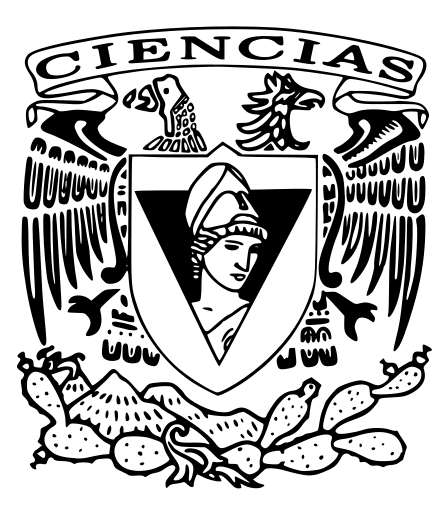
\includegraphics[width=0.5\textwidth]{escudo_f-ciencias.png}
	\vfill

% Bottom of the page
	{\large Jueves 30 de Agosto del 2018 \par}
\end{titlepage}

\pagebreak
\setlength{\voffset}{-0.75in}
\setlength{\headsep}{5pt}

%\newcommand{\ed}[2]{(#1) edge (#2)}
%\newcommand{\eee}[4]{\path [->,draw,thin] ($ (#1) !.5! (#2)$) -- ($ (#3) !.5! (#4) $);}

\newcommand{\is}[1]{V_{\{B, x, r\}}}

\begin{enumerate}
	%Ejercicio 1
	\item {
		Dados los procesos $A$ y $B$, diseña un algoritmo para el ataque coordinado
		proximado (aproximate agreement) en el que para llegar al acuerdo deben
		decidir	valores que estén a distancia a lo más $\frac{1}{2^k}$ y utilice menos
		rondas de comunicación que el algoritmo visto en clase.\\

		El algoritmo propuesto es el siguiente:\\

		\begin{algorithmic}[1]
			\Require $id \in \{A,B\},\ init \in \{0, 1\},\ k \in \mathbb{N}$
			\Ensure $v_A^k\ \& \ v_B^k$ tales que $|v_A^k\ - \ v_B^k|\ \leq\ \dfrac{1}
				{2^k}$
			\Function{\textbf{ Modelo:}$\{A\leftrightarrow B, A \rightarrow B, 
				A \leftarrow B\}$}{$init$}			
				\State $v\ \leftarrow init$
				\For{r = 0 \textbf{to} k + 1}{}
					\State $send(v)$
					\State $msg \leftarrow$ receive()
					\If{$msg \ne null$}
						\If{$msg = v$}
							\State break
						\Else	
							\State $v \leftarrow \dfrac{v + msg}{2}$
						\EndIf
					\EndIf
				\EndFor
				\State \Return$v$
			\EndFunction
		\end{algorithmic}
	}
	

	\textbf{Demostración:}\\
	S.P.G. proponemos a la variable $\is{B}$ dónde $V$ representa la
	invariante de ciclo y el vector $\{B, x, r\}$ en el subíndice representa el
	nombre del proceso, su	valor actual y el número de ronda actual
	respectivamente.\\\\
	Por el teorema visto con Karla en clase sabemos que en la ronda $r$ hay
	comunicación perfecta, entonces $\ v_A^k\  =\  v_B^k\ $ en la ronda $r + 1$.\\
	


	%Ejercicio 2
	\item {
		Dibuja la gráfica del protocolo que diseñaste para 2 rondas para $k = 2$.
		Para cada vértice indica el valor de salida y para cada arista indica el
		patrón de mensajes recibidos.\\\\

		\begin{tikzpicture}[scale = 1.4]
			\tikzstyle{every node} = [draw, shape = circle]
			\foreach \i/\s in {0/$A \longrightarrow B$, 6/$A\longleftarrow B$}{
				\node at (\i, 9) (Bu\i) [label = above : {1}] {$B$};
				\node at (\i + 3, 9) (Au\i) [label = above : {1}] {$A$};
				\ifthenelse{\i = 6}{\draw (Au0) -- node[rectangle,above,draw=none]{$A\longleftrightarrow B$}++(Bu\i);}{}
				\draw (Au\i) --node[rectangle, above, draw=none, label = above : {\s}]{\s}++ (Bu\i) ;
				\node at (\i, 0) (Al\i) [label = below : {0}] {$A$};
				\node at (\i + 3, 0) (Bl\i) [label = below : {0}] {$B$};
				\ifthenelse{\i = 6}{\draw (Bl0) -- node[rectangle, below, draw=none]{$A\longleftrightarrow B$}++ (Al\i);}{}
				\draw (Al\i) --node[rectangle, below, draw=none, label = below : {\s}]{\s}++ (Bl\i);
			}
			\foreach \i/\j/\k/\s/\c in {2/0/3, 4/2/2, 6/4/2, 8/6/1}{
				\node at (0, \i) (Ai\i) [label = left : {\k/4}] {$A$};
				\node at (0, \i - 1) (Bi\i) [label = left : {\k/4}] {$B$};
				\ifthenelse{\i > 2}{\draw (Ai\j) -- (Bi\i);}{}
				\draw (Ai\i) -- (Bi\i);
				\node at (9, \i - 1) (Ad\i) [label = right : {\k/4}] {$A$};
				\node at (9, \i) (Bd\i) [label = right : {\k/4}] {$B$};
				\ifthenelse{\i > 2}{\draw (Bd\j) -- (Ad\i);}{}
				\draw (Ad\i) -- (Bd\i);
			}
		\end{tikzpicture}
	}


\end{enumerate}
\end{document}